\documentclass{article}
\usepackage{fancyhdr} 
\usepackage{lastpage}
\usepackage{mathtools}
\usepackage{extramarks}
\usepackage{graphicx}
\usepackage{listings}
\usepackage{courier}
\usepackage{lipsum} 
\usepackage{enumerate}
\usepackage{amsmath}
\usepackage{url}
\usepackage{caption}

\lstset{
  language=XML,
  morekeywords={encoding,
    xs:schema,xs:element,xs:complexType,xs:sequence,xs:attribute}
}

% Margins
\topmargin=-0.45in
\evensidemargin=0in
\oddsidemargin=0in
\textwidth=6.5in
\textheight=9.0in
\headsep=0.25in
\linespread{1.1} % Line spacing

% Set up the header and footer
\pagestyle{fancy}
\lhead{COMP3308}
\chead{Introduction to Artificial Intelligence}
\rhead{Assignment 2}
\lfoot{}
\cfoot{\thepage}
\rfoot{Woo Hyun Jung 310250811 \\  Khanh Cao Quoc Nguyen 311253865} 
\renewcommand\headrulewidth{0.4pt}
\renewcommand\footrulewidth{0.4pt}
\renewcommand{\tt}{\texttt}
\setlength\parindent{0pt} 

\title{COMP3308 Assignment 2 \\ Bayesian Networks}
\author{Woo Hyun Jung 310250811 \\  Khanh Cao Quoc Nguyen 311253865}
\date{}
\begin{document}
\maketitle
\thispagestyle{empty}
\newpage

\section{Aim}
The aim of this assignment is to build Bayesian networks for diagnostic problems and verify the independence statements by using existing tools such as JavaBayes and implementing an inference algorithm to compute posterior probabilities.

\section{Methods}
\subsection{Bayesian Networks}
Bayesian networks are simple, probabilistic graphical models that represent sets of random variables and their conditional dependencies.

\subsection{Variable Elimination}
blah blah blah blah blah blah blah blah blah blah blah blah blah blah blah blah blah blah blah blah blah blah blah blah blah blah blah blah blah blah blah blah blah blah blah blah blah blah blah blah blah blah blah blah blah blah blah blah blah blah blah blah blah blah blah blah blah blah blah blah blah blah blah blah blah blah blah blah blah blah blah blah blah blah blah blah blah blah blah blah blah blah blah blah blah blah blah blah blah blah blah blah blah 

\subsection{Likelihood Weighting}
blah blah blah blah blah blah blah blah blah blah blah blah blah blah blah blah blah blah blah blah blah blah blah blah blah blah blah blah blah blah blah blah blah blah blah blah blah blah blah blah blah blah blah blah blah blah blah blah blah blah blah blah blah blah blah blah blah blah blah blah blah blah blah blah blah blah blah blah blah blah blah blah blah blah blah blah blah blah blah blah blah blah blah blah blah blah blah blah blah blah blah blah blah 

\section{Results and Discussion}
\subsection{Question 1}

Metastatic cancer is a possible cause of a brain tumour and is also an explanation for increased total serum calcium. In turn, either of these could explain a patient falling into a coma. Severe headache is also possibly associated with a brain tumour. 

\begin{itemize}
\item The prior probability of metastatic cancer $P(m)$ is 0.2. 
\item The conditional probability of increased total serum calcium $P(I | M)$ is: $P(i | m) = 0.8$ and $P(i | \neg m) = 0.2$ 
\item The conditional probability of brain tumor $P(B | M)$ is: $P(b | m) = 0.2$ and $P(b | \neg m) = 0.05$ 
\item The conditional probability of coma $P(C | I, B)$ is: $P(c | i, b) = 0.8$, $P(c | \neg i, b) = 0.8$, $P(c | i, \neg b) = 0.8$ and $P(c | \neg i, \neg b) = 0.05$. 
\item The conditional probability of severe headache $P(S | B)$ is $P(s | b) = 0.8$ and $P(s | �b) = 0.6$.
\end{itemize} 

\begin{enumerate}[a)]
\item Construct and show the equivalent graphical model.
\begin{figure}
\begin{center}
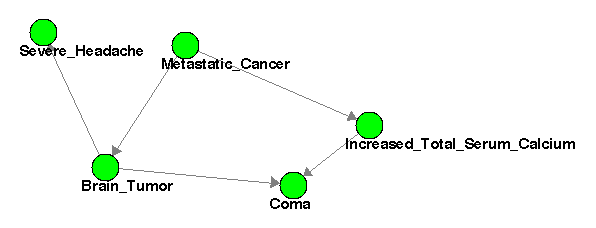
\includegraphics[scale=0.7]{part1_bn}
\caption{Equivalent graphical model created using JavaBayes}
\end{center}
\end{figure}

\item What is the prior probability of coma $P(C)$?

\begin{minipage}{\linewidth}
\begin{lstlisting}
Posterior distribution:
	probability (  "Coma" ) { //1 variable(s) and 2 values
		table 
			0.32	// p(true | evidence )
			0.68; 	// p(false | evidence );
	}
\end{lstlisting}
\captionof{figure}{Probability of coma query output using JavaBayes}
\end{minipage}\\
\\
\\
Using the \tt{Query} function in JavaBayes, $P(C) = 0.32$.

\item What is the probability of metastatic cancer given the patient has severe headaches and has not fallen into coma? 

\begin{minipage}{\linewidth}
\begin{lstlisting}
Posterior distribution:
	probability (  "Metastatic_Cancer" ) { //1 variable(s) and 2 values
		table 
			0.12087912087912088	// p(true | evidence )
			0.8791208791208791; 	// p(false | evidence );
	}
\end{lstlisting}
\captionof{figure}{$P(M | S, \neg C)$ query output using JavaBayes}
\end{minipage}\\
\\
\\
Using the \tt{Observe} and \tt{Query} functions in JavaBayes, $P(M | S, \neg C) = 0.12087912087912088$.

\item What is the Markov blanket of coma?

In a Bayesian network, the Markov blanket of node A includes its parents, children and the other parents of all of its children.

Therefore the Markov blanket of coma are brain tumor and increased total serum calcium.

\item Are increased total serum calcium and brain tumor independent given coma? Explain.

No, because of explaining away otherwise known as Berkson's Paradox.

Normally, total serum calcium and brain tumor are independent, but if we are given coma they become dependent since they share the same child.

\item What is the probability of fallen into coma given the patient has metastatic cancer? 

\begin{minipage}{\linewidth}
\begin{lstlisting}
Posterior distribution:
	probability (  "Coma" ) { //1 variable(s) and 2 values
		table 
			0.68	// p(true | evidence )
			0.32; 	// p(false | evidence );
	}
\end{lstlisting}
\captionof{figure}{$P(C | M)$ query output using JavaBayes}
\end{minipage}\\
\\
\\
Using the \tt{Observe} and \tt{Query} functions in JavaBayes, $P(C | M) = 0.68$.
\end{enumerate} 

\subsection{Question 2}
\begin{minipage}{\linewidth}
\begin{center}
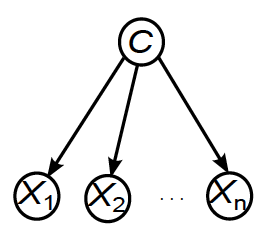
\includegraphics[scale=0.5]{part2_nbc}
\end{center}
\captionof{figure}{Naive Bayes Classifer}
\end{minipage}\\

\begin{enumerate}[a)]
\item 

$$ P(C | x_1, ... , x_n) = \frac{P(C) P(x_1, ... , x_n | C)}{P(x_1, ... , x_n)} $$ Bayes' Theorem


$$ P(C | x_1, ... , x_n)  = \frac{P(C, x_1, ... , x_n)}{P(x_1, ... , x_n)} $$ Conditional Probability
$$ P(C | x_1, ... , x_n) P(x_1, ... , x_n) = P(C, x_1, ... , x_n) $$

$$ P(C, x_1, ... , x_n) =  P(x_1, ... , x_n) \frac{P(C) P(x_1, ... , x_n | C)}{P(x_1, ... , x_n)}$$
$$ P(C, x_1, ... , x_n) =  P(C) P(x_1, ... , x_n | C)$$  

$$P(x_1, ... , x_n | C) =  \prod_{i=1}^n P(x_i | C)$$ which is the distribution for $x_1, ..., x_n$ which can be given by the product of each node's probability given it's parent which is $C$.


Therefore,
$$P(C, x_1, ... , x_n) =  P(C) \prod_{i=1}^n P(x_i | C) $$

\end{enumerate}

\subsection{Question 3}
something something diagnosis

\subsection{Question 4}
\subsubsection{Likelihood Weighting}

We implemented the likelihood weighting in Python 2.7.5 to calculate the probability of $P(cloudy | sprinkler, wetgrass)$. \\

Our program takes in the number of samples used to construct the estimate (N) as input and then runs M times which is set to 1000 by default. It then returns the mean, variance and standard deviation of the probability calculated using the likelihood weighting algorithm.\\

Below in Table 1, are the results for N=10, 100, 1000, 5000.

\begin{table}[h]
\centering
\begin{tabular}{|c|c|c|c|}
\hline
N    & Mean      & Variance        & Standard Deviation \\ \hline
10   & 0.5069    & 0.02524239      & 0.158878538513     \\ \hline
100  & 0.50004   & 0.0025593984    & 0.0505904971314    \\ \hline
1000 & 0.499573  & 0.000222700671  & 0.0149231588814    \\ \hline
5000 & 0.5001358 & 4.979223836e-05 & 0.00705636155253   \\ \hline
\end{tabular}
\caption {Accuracy results for likelihood weighting}
\end{table}

blah blah blah blah blah blah blah blah blah blah blah blah blah blah blah blah blah blah blah blah blah blah blah blah blah blah blah blah blah blah blah blah blah blah blah blah blah blah blah blah discuss table?

\subsubsection{Exact Inference using JavaBayes}
\begin{minipage}{\linewidth}
\begin{center}
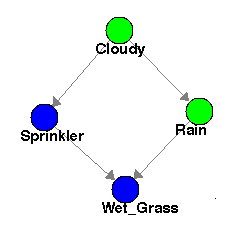
\includegraphics[scale=0.7]{part4_bn}
\end{center}
\captionof{figure}{Equivalent graphical model created using JavaBayes. Sprinkler and Wet Grass set to true.}
\end{minipage}\\

\begin{minipage}{\linewidth}
\begin{lstlisting}
Posterior distribution:
	probability (  "Cloudy" ) { //1 variable(s) and 2 values
		table 
			0.17475728155339806	// p(true | evidence )
			0.825242718446602; 	// p(false | evidence );
	}
\end{lstlisting}
\captionof{figure}{$P(Cloudy | Sprinkler, WetGrass )$ query output using JavaBayes}
\end{minipage}\\
\\
\\

blah blah blah blah blah blah blah blah blah blah blah blah blah blah blah blah blah blah blah blah blah blah blah blah blah blah blah blah blah blah blah blah blah blah blah blah blah blah blah discuss exact inference and compare to other thing

\section{Conclusions}
blah blah blah blah blah blah blah blah blah blah blah blah blah blah blah blah blah blah blah blah blah blah blah blah blah blah blah blah blah blah blah blah blah blah blah blah blah blah blah blah blah blah blah blah blah blah blah blah blah blah blah blah blah blah blah blah blah blah blah blah blah blah blah blah blah blah blah blah blah blah blah blah blah blah blah blah blah blah blah blah blah blah blah blah blah blah blah blah blah blah blah blah blah 

\section{Reflection}
blah blah blah blah blah blah blah blah blah blah blah blah blah blah blah blah blah blah blah blah blah blah blah blah blah blah blah blah blah blah blah blah blah blah blah blah blah blah blah blah blah blah blah blah blah blah blah blah blah blah blah blah blah blah blah blah blah blah blah blah blah blah blah blah blah blah blah blah blah blah blah blah blah blah blah blah blah blah blah blah blah blah blah blah blah blah blah blah blah blah blah blah blah 

\section{Code}
Our implementation of Likelihood Weighting was written in Python 2.7.5.\\

This implementation was designed to work with any Bayesian network and not just the Cloudy-Rain-Sprinkler-WetGrass network.

\subsection{XML Format}
The program reads an XML file which has the structure of the network and probability values and makes the appropriate data structures.\\

The XML of the Cloudy-Rain-Sprinkler-WetGrass network can seen in the figure below.

\begin{minipage}{\linewidth}
\begin{lstlisting}
<network>
	<node>
		<id>C</id>
		<name>Cloudy</name>
		<probability>0.5</probability>
	</node>

	<node>
		<id>S</id>
		<name>Sprinkler</name>
		<parent>C</parent>
		<probability given="C">0.1</probability>
		<probability given="-C">0.5</probability>
	</node>
	
	<node>
		<id>R</id>
		<name>Rain</name>
		<parent>C</parent>
		<probability given="C">0.8</probability>
		<probability given="-C">0.2</probability>
	</node>
	
	<node>
		<id>W</id>
		<name>Wet Grass</name>
		<parent>S</parent>
		<parent>R</parent>
		<probability given="S,R">0.99</probability>
		<probability given="S,-R">0.9</probability>
		<probability given="-S,R">0.9</probability>
		<probability given="-S,-R">0.00</probability>
	</node>
</network>
\end{lstlisting}
\captionof{figure}{Cloudy-Rain-Sprinkler-WetGrass-Network.xml}
\end{minipage}\\

\subsection{Instructions}
To run our implementation, change directory to the where the code is. Make sure that Cloudy-Rain-Sprinkler-WetGrass-Network.xml file is present.\\
\\
Then run:

\begin{lstlisting}
python likelihood.py <N>
\end{lstlisting}
where N is the number of samples used.\\

\subsubsection{Example}
\begin{lstlisting}
$ python likelihood.py 1000
----------- Likelihood Weighting Sampling ---------------
Estimating the probability of P(Cloudy | Sprinkler, Wetgrass)
---- Summary ----
N: 1000
M: 1000
Mean: 0.499573
Variance: 0.000222700671
Standard Deviation: 0.0149231588814

\end{lstlisting}












\end{document}